\documentclass[a4paper, spanish]{article}

\usepackage[T1]{fontenc}
\usepackage[utf8]{inputenc}
\usepackage{babel} % , parskip
\usepackage[colorlinks]{hyperref}
\usepackage{graphicx}
\usepackage{tikz}
\usetikzlibrary{babel, chains}

\title{Projectizer (SAR)\\ Documento de Análisis}
\author{Version 1.0 \\ M. Blanc, L.C. Jariego, P. Marcos, F. Martín, D. Nevado}

\begin{document}

\maketitle
\begin{abstract}
Este documento comprende la etapa de analisis de \textit{Projectizer}, un Sistema de Análisis de Requisitos (SAR) cuyo objetivo es servir de herramienta de gestión de requisitos en proyectos. La herramienta esta destinada a empresas de desarrollo de software que adopten la metodología Scrum, o similar.

\end{abstract}
\vspace{\fill}
\tableofcontents
\let\oldsection\section\renewcommand\section{\clearpage\oldsection}

\section{Descripción del Sistema}
\subsection{Descripción y Motivación}
El objetivo principal del proyecto es proporcionar una herramienta de administración y consulta de requisitos a directores de proyecto e ingenieros y, adicionalmente, brindar una forma de comunicación más inmediata con los clientes a los que se dé acceso.
Con el uso de la herramienta, se espera aumentar las posibilidades de éxito de un proyecto.


\subsection{Objetivos del Sistema}
% Esta descripcion esta tomada practicamente palabra-a-palabra del Anexo 1
% (Seccion A1. Contexto). Para que reescribirlo cuando ya esta perfectamente
% bien redactado exactamente lo que quieren?
El sistema SAR esta dirigido a empresas que realizan proyectos de desarrollo de
software. Se trata de una herramienta que permite administrar los requisitos
de sus proyectos, facilitando la comunicación entre el grupo de trabajo y los
clientes y evitando los problemas que generalmente se presentan cuando se realizan
cambios sobre la especificación de requisitos.

\subsection{Usuarios del Sistema}\label{sec:usuarios}
Hemos identificado 3 tipos diferentes de usuarios del sistema:
\begin{description}
  \item [Cliente] un cliente de la empresa que contrata un proyecto.
  \item [Jefe de Proyecto] el encargado en la empresa de gestionar proyectos.
  \item [Ingeniero] los trabajadores en la empresa que llevaran a cabo el trabajo.
\end{description}

\section{Definición del Sistema}
Ya descrito el sistema a grandes rasgos, en esta sección se concretan algunos
aspectos del sistema.

\subsection{Modelado de Casos de Uso}
\begin{figure}[h!]
\centering
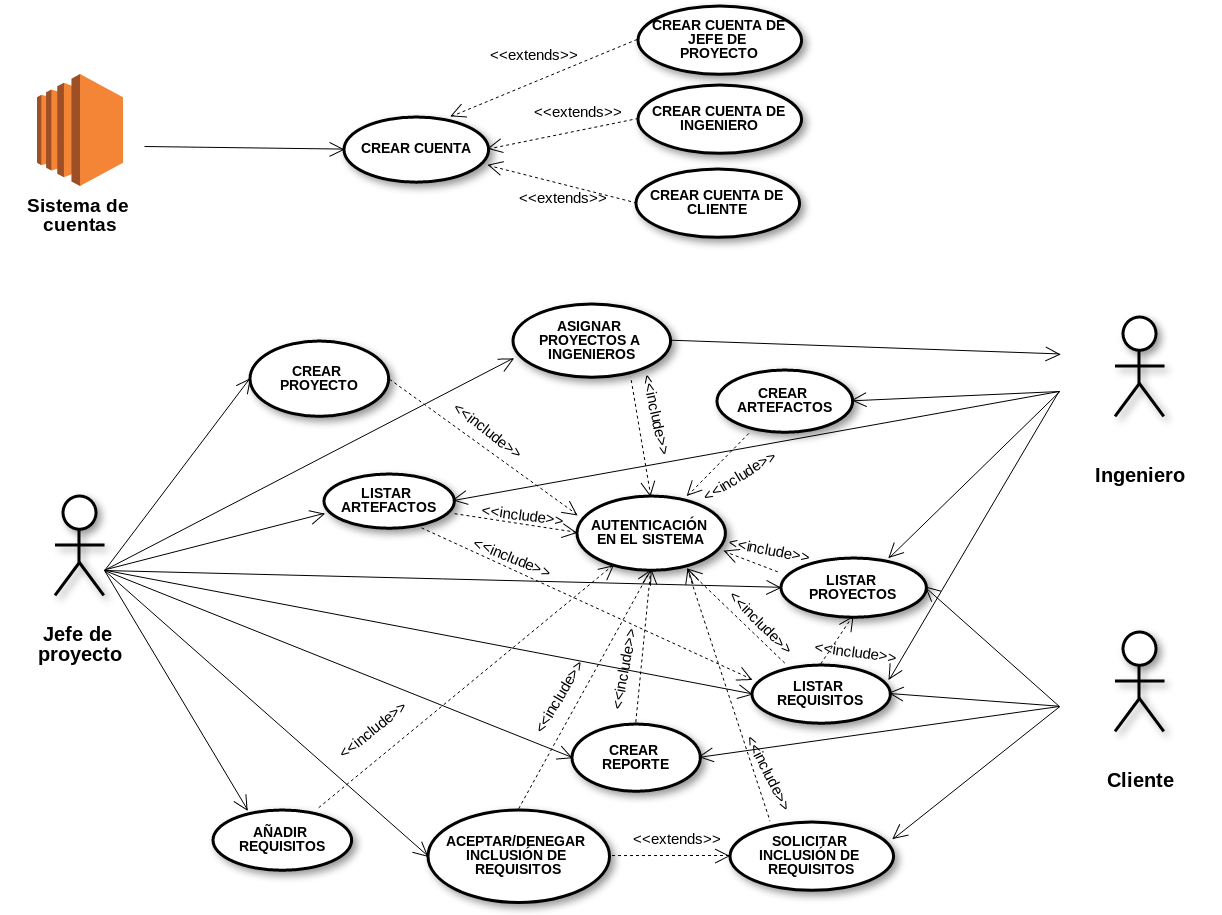
\includegraphics[width=0.9\textwidth]{diagramas/diagrama-casos-uso.png}
\caption{Diagrama de casos de uso}\label{fig:casosdeuso}
\end{figure}
En primer lugar, hemos separado el sistema de cuentas para no sobrecargar
demasiado el diagrama principal.
Se deben poder crear 3 tipos distintos de cuentas para los tres tipos de usuarios 
del sistema (véase la \autoref{sec:usuarios}).

La siguiente malla del diagrama de casos de uso une a cada rol con las acciones
que puede efectuar en el sistema. Los elementos mas destacables son los siguientes:
\begin{itemize}
  \item Todas las acciones necesitan que el usuario este autenticado en el sistema, por lo que todas las acciones incluyen \textit{Autenticación en el sistema}.
  De este modo, se limita el acceso a las acciones que tiene cada rol.
  \item La acción de \textit{Listar Requisitos} incluye listar proyectos, ya que los requisitos siempre van a estar asignados a un proyecto que se debe seleccionar previamente.
\end{itemize}

\subsection{Requisitos del sistema}
En esta sección, se recogen los requisitos del sistema de manera más concreta.

\newcommand{\CasoDeUso}[1]{%
\pgfqkeys{/ings/analisis}{%
  define/.style = { ##1/.initial = \textcolor{red}{(Unset {##1})}, },
  define/.list = {%
    identificador,autor,
    fecha,actores involucrados,resumen,precondiciones,
    postcondiciones,secuencia,caminos alternativos,
    clases involucradas,
  },
  #1,
  /utils/exec = {%
    \noindent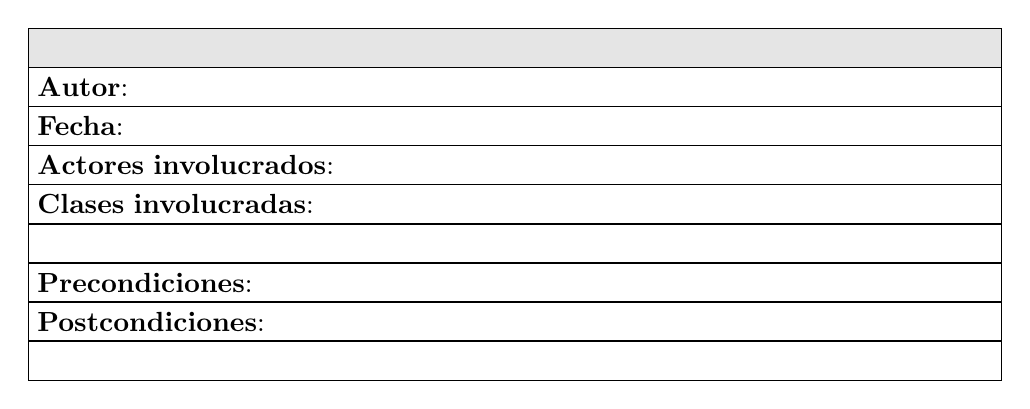
\begin{tikzpicture}[%
        my node/.style = {%
          text width=\textwidth,
          on chain,
          minimum height = 0.5cm,
          draw = black,
        },
        start chain = going below,
        node distance = -0.5pt,
      ]
      \node[my node, fill=black!10, align=center] (id)       {\pgfkeysvalueof{/ings/analisis/identificador}};
      \node[my node] (autor)    {\textbf{Autor}: \pgfkeysvalueof{/ings/analisis/autor}};
      \node[my node] (fecha)    {\textbf{Fecha}: \pgfkeysvalueof{/ings/analisis/fecha}};
      \node[my node] (actores)  {\textbf{Actores involucrados}: \pgfkeysvalueof{/ings/analisis/actores involucrados}};
      \node[my node] (clases) {\textbf{Clases involucradas}: \pgfkeysvalueof{/ings/analisis/clases involucradas}};
      \node[my node, align=justify] (resumen) {\pgfkeysvalueof{/ings/analisis/resumen}};
      \node[my node] (precondiciones) {\textbf{Precondiciones}: \pgfkeysvalueof{/ings/analisis/precondiciones}};
      \node[my node] (postcondiciones) {\textbf{Postcondiciones}: \pgfkeysvalueof{/ings/analisis/postcondiciones}};
      \node[my node] (secuencia) {\pgfkeysvalueof{/ings/analisis/secuencia}};
    \end{tikzpicture}
    %\begin{itemize}
    %\item secuencia             \pgfkeysvalueof{/ings/analisis/secuencia}
    %\item caminos alternativos  \pgfkeysvalueof{/ings/analisis/caminos alternativos}
    %\end{itemize}
  }
}}

\CasoDeUso{%
  identificador          = {CrearProyectos},
  autor                  = {Fernando Martín},
  fecha                  = {2018-03-01},
  actores involucrados   = {Jefe de Proyecto},
  resumen                = {Acción que permite a un Jefe de Proyecto crear un proyecto.},
  precondiciones         = {Log In, no debe existir un proyecto con ese nombre},
  postcondiciones        = {Se crea un proyecto},
  secuencia = {%
    \begin{itemize}
    \item \textbf{Usuario}: Rellena formulario: nombre proyecto, descripción del proyecto, cliente, ingenieros.
    \item \textbf{Sistema}: Muestra dialogo de confirmación.
    \item \textbf{Usuario}: Confirma la creación.
    \item \textbf{Sistema}: Redirige a la página de información del proyecto y envía un correo a las partes involucradas para notificarles de que han sido añadidos a un proyecto nuevo.
    \end{itemize}
  },
  caminos alternativos   = {El nombre es invalido},
  clases involucradas    = {JefeDeProyecto, Proyecto},
}

\pagebreak\CasoDeUso{%
  identificador          = {CrearRequisitos},
  autor                  = {Fernando Martín},
  fecha                  = {2018-03-01},
  actores involucrados   = {Jefe de Proyecto},
  resumen                = {Acción que permite a un jefe de proyecto crear requisitos y asignarlas a un proyecto previamente creado.},
  precondiciones         = {Log In, el jefe de proyecto ha creado el proyecto previamente},
  postcondiciones        = {El proyecto tiene un nuevo requisito asociado a él.},
  secuencia = {%
    \begin{itemize}
    \item \textbf{Usuario}: Selecciona el proyecto
    \item \textbf{Sistema}: Muestra información relativa al proyecto.
    \item \textbf{Usuario}: Pulsa en crear requisito.
    \item \textbf{Sistema}: Muestra un formulario.
    \item \textbf{Usuario}: Rellena el formulario.
    \item \textbf{Sistema}: Muestra el requisito añadido al proyecto.
    \end{itemize}
  },
  caminos alternativos   = {No hay ningún proyecto con el cliente. No rellena algún campo del formulario},
  clases involucradas    = {JefeDeProyecto, Proyecto, Requisito},
}

\pagebreak\CasoDeUso{%
  identificador          = {CrearSolicitudes},
  autor                  = {Fernando Martín},
  fecha                  = {2018-03-01},
  actores involucrados   = {Cliente},
  resumen                = {Acción que permite a un cliente crear una solicitud para añadir o cambiar un requisito de un proyecto.},
  precondiciones         = {Log in, el cliente esta al menos en un proyecto},
  postcondiciones        = {El jefe de proyecto recibe una solicitud  que puede aceptar o rechazar},
  secuencia = {%
    \begin{itemize}
    \item \textbf{Usuario}: Busca proyecto.
    \item \textbf{Sistema}: Muestra información del proyecto.
    \item \textbf{Usuario}: Selecciona crear solicitud.
    \item \textbf{Sistema}: Muestra el formulario.
    \item \textbf{Usuario}: Rellena el formulario.
    \item \textbf{Sistema}: Valida e inserta los datos en la base de datos.
  \end{itemize}
  },
  caminos alternativos   = {Error en el formulario, no rellenar campos obligatorios},
  clases involucradas    = {Cliente, Solicitud, Proyecto},
}
%
\pagebreak\CasoDeUso{%
  identificador          = {CrearArtefactos},
  autor                  = {Fernando Martín},
  fecha                  = {2018-03-01},
  actores involucrados   = {Ingeniero},
  resumen                = {Esta acción permite a un ingeniero crear a un ingeniero un artefeacto y añadirlo a un requisito de un proyecto..},
  precondiciones         = {Log In, el ingeniero esta asignado a este proyecto, y existe al menos un requisito proyecto},
  postcondiciones        = {Se ha añadido un artefacto al requisito elegido del proyecto},
  secuencia = {%
    \begin{itemize}
    \item \textbf{Usuario}: Busca un proyecto al que este adscrito.
    \item \textbf{Sistema}: Muestra la lista de proyectos.
    \item \textbf{Usuario}: Elige un proyecto.
    \item \textbf{Sistema}: Muestra la información del proyecto.
    \item \textbf{Usuario}: Elige un requisito.
    \item \textbf{Sistema}: Muestra la información del requisito.
    \item \textbf{Usuario}: Pulsa añadir artefacto.
    \item \textbf{Sistema}: Muestra un formulario.
    \item \textbf{Usuario}: Rellena el formulario.
    \item \textbf{Sistema}: Confirma que se ha añadido.
    \end{itemize}
  },
  caminos alternativos   = {El ingeniero no esta en ningún proyecto, el proyecto no tiene requisito, el formulario no se rellena bien.},
  clases involucradas    = {Ingeniero, Proyecto, Requisito, Artefacto},
}

\pagebreak% Mejor poner un pagebreak aqui para separar secciones logicas
\subsection{Maquetas}
Como parte del documento de análisis, incluimos varias maquetas para ilustrar
distintos casos de uso junto con su funcionamiento interno.

La pagina principal de un proyecto muestra el estado de las tareas. Se usan distintos
colores para remarcar el estado de cada tarea. A la izquierda del todo se sitúan las historias de usuario, y a la derecha del todo están los impedimentos.
\begin{figure}[h!]
\centering
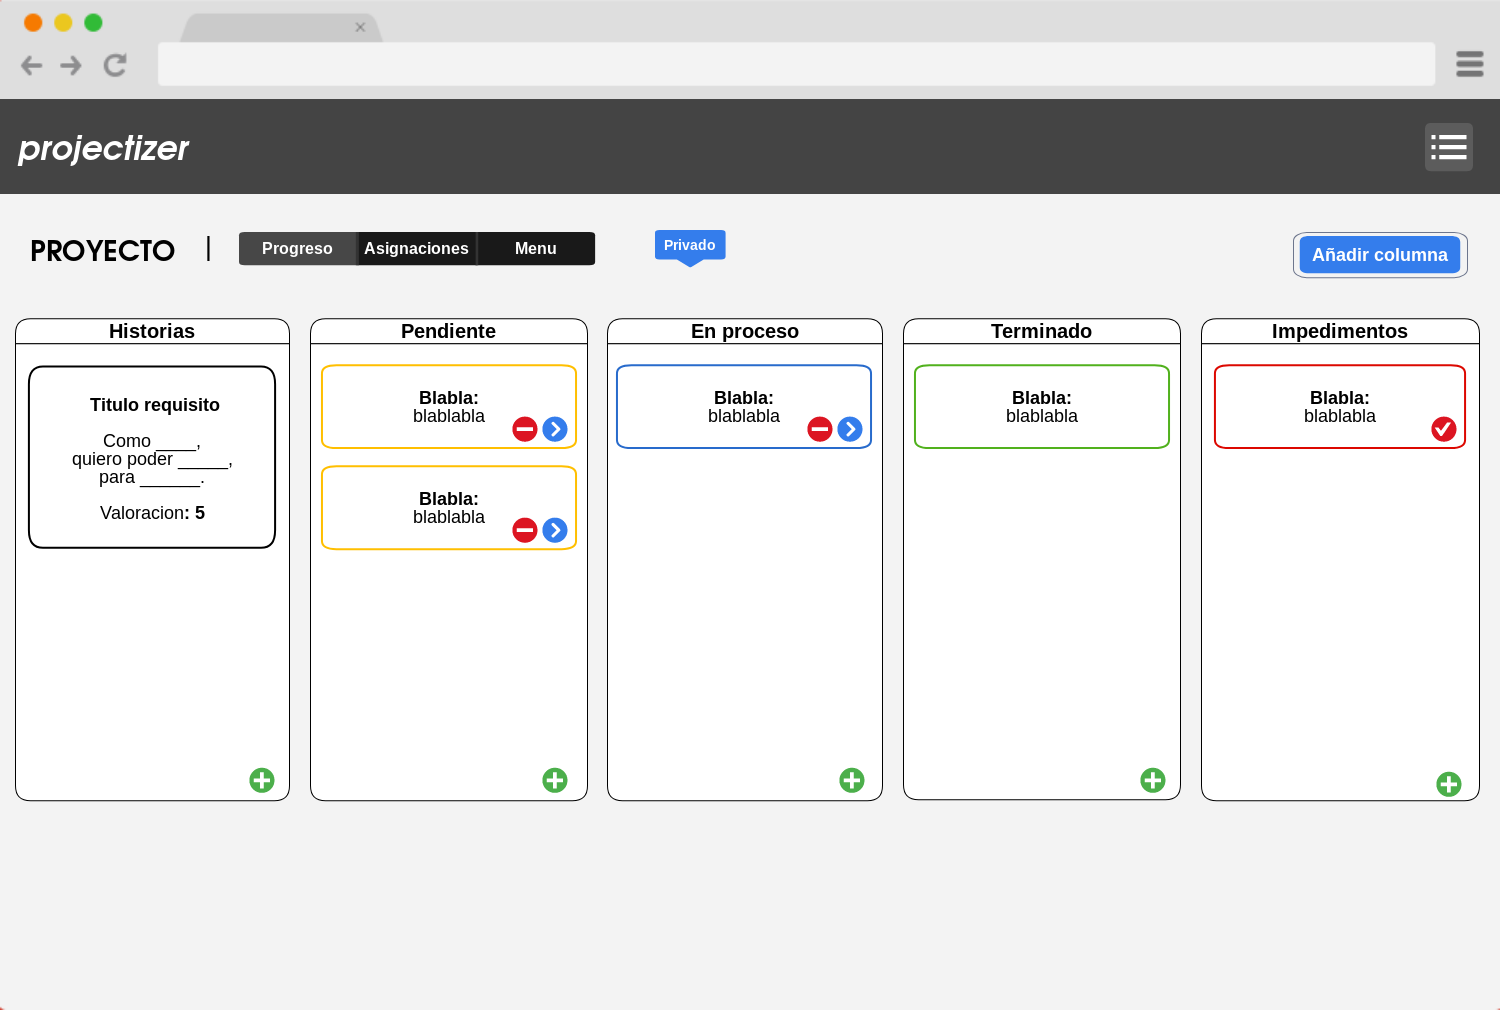
\includegraphics[width=0.7\textwidth]{maquetas/home.png}
\caption{Vista de la pagina principal de un proyecto}\label{fig:maquetahome}
\end{figure}

Los jefes de proyecto tienen acceso a un formulario para crear proyectos nuevos.
y pre-asignar ingenieros y clientes.
\begin{figure}[h!]
\centering
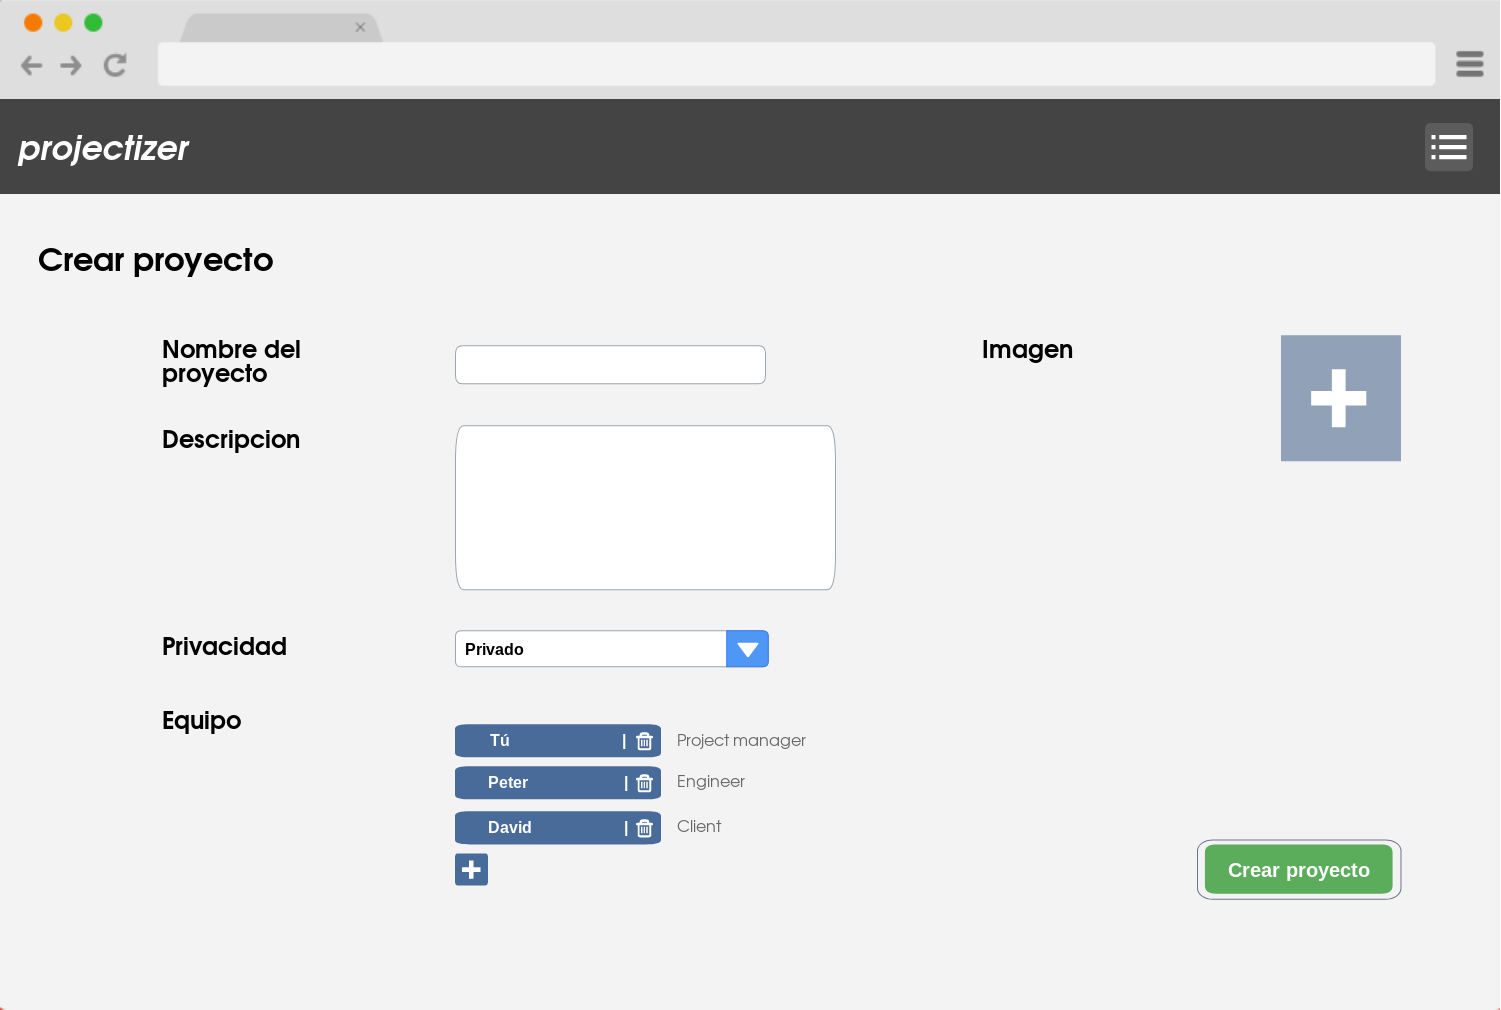
\includegraphics[width=0.7\textwidth]{maquetas/proyecto.png}
\caption{Formulario de crear proyecto}\label{fig:maquetaproyecto}
\end{figure}

A continuación se muestra el dialogo para añadir nuevos requisitos a un proyecto.
\begin{figure}[h!]
\centering
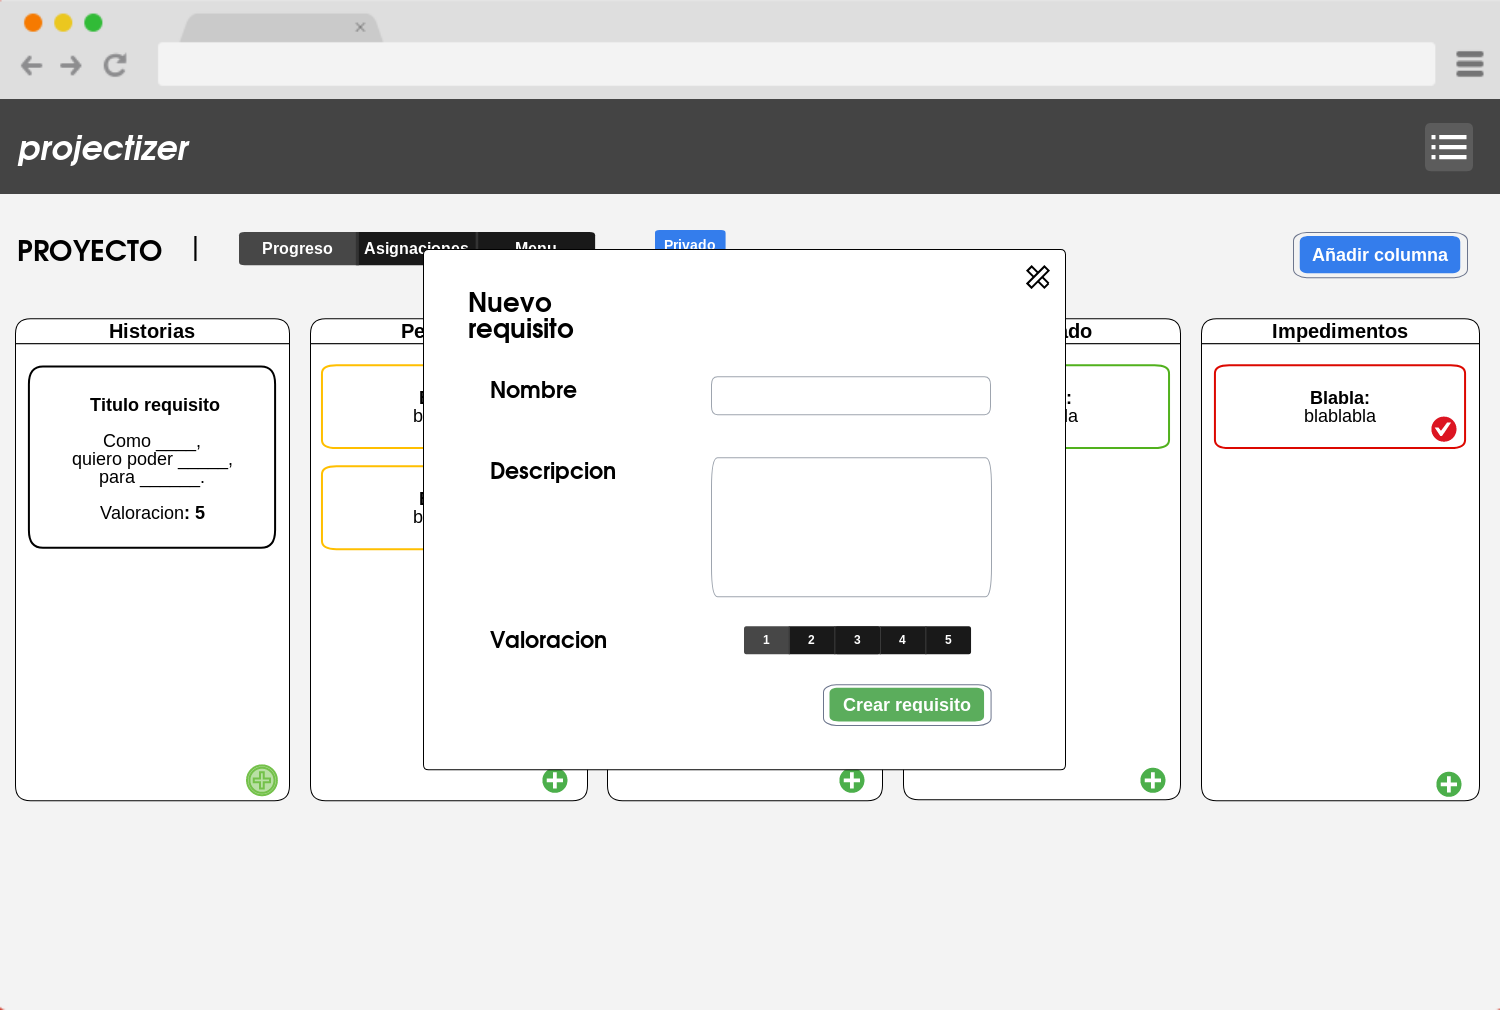
\includegraphics[width=0.7\textwidth]{maquetas/requisitos.png}
\caption{Dialogo modal de añadir requisito}\label{fig:maquetarequisito}
\end{figure}

Para solicitar un nuevo requisito, un cliente debe cumplimentar el siguiente formulario.
\begin{figure}[h!]
\centering
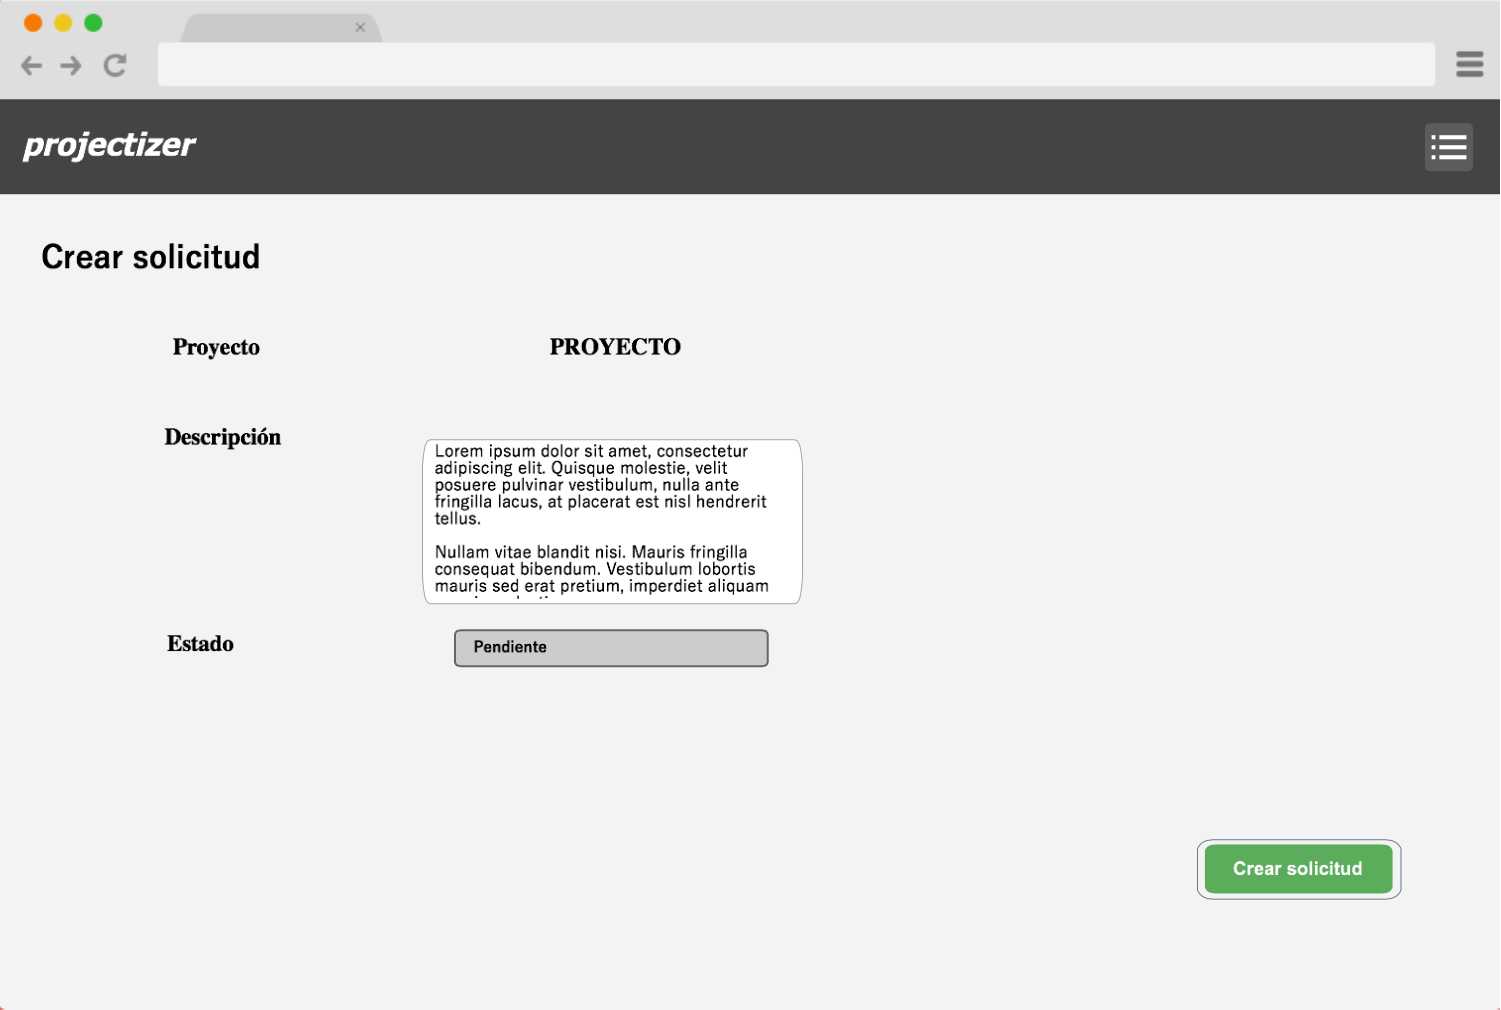
\includegraphics[width=0.7\textwidth]{maquetas/solicitudes.png}
\caption{Formulario de solicitud de un requisito}\label{fig:maquetasolicitud}
\end{figure}

Finalmente, mostramos el formulario que puede usar un ingeniero para subir un artefacto a la plataforma.
\begin{figure}[h!]
\centering
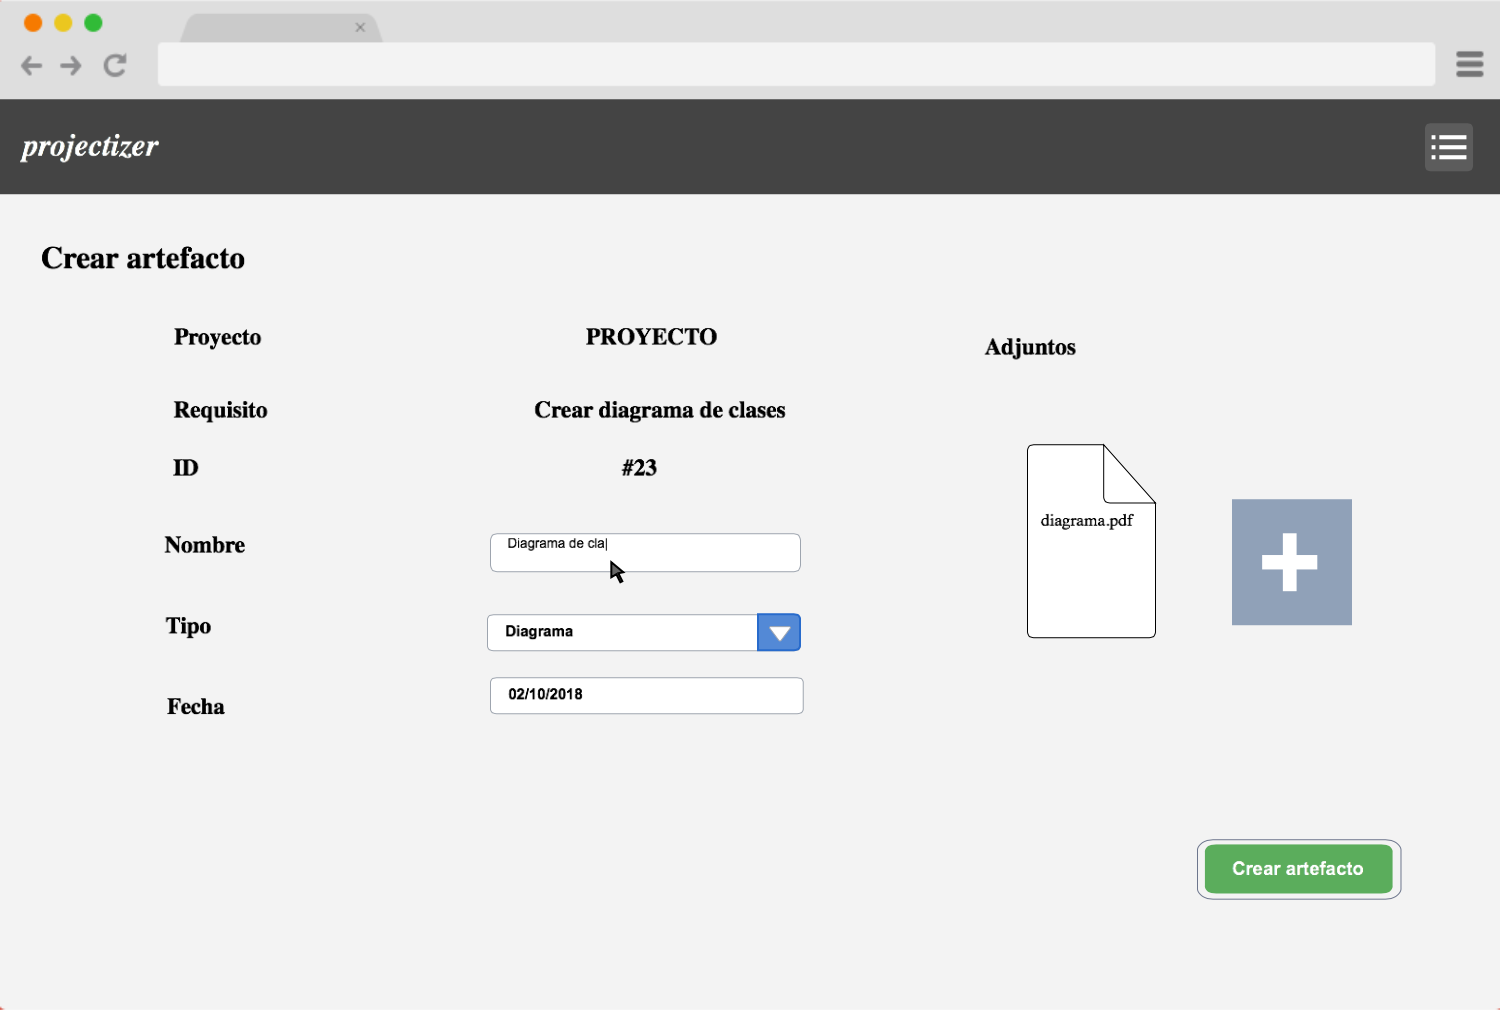
\includegraphics[width=0.7\textwidth]{maquetas/artefactos.png}
\caption{Formulario de crear artefacto}\label{fig:maquetaartefacto}
\end{figure}

\section{Glosario}
\begin{description}
  \item [SAR] Abreviación de Sistema de Análisis de Requisitos
  \item [JdP] Abreviación de Jefe de Proyecto
  \item [Solicitud] Se refiere implícitamente a una solicitud de un requisito nuevo
  \item [Artefacto] Un producto tangible producido durante el desarrollo.
  \item [Scrum] Metodología de desarrollo ágil comercial. 
\end{description}

\end{document}

